%% Phase 4 research paper -- Springer Nature template (sn-jnl, sn-basic style)
\documentclass[pdflatex,sn-basic,Numbered,iicol]{sn-jnl}

\usepackage{graphicx}
\usepackage{multirow}
\usepackage{amsmath,amssymb,amsfonts}
\usepackage{amsthm}
\usepackage{mathrsfs}
\usepackage[title]{appendix}
\usepackage{xcolor}
\usepackage{textcomp}
\usepackage{manyfoot}
\usepackage{booktabs}
\usepackage{array}
\usepackage{tabularx}
\usepackage{algorithm}
\usepackage{algorithmicx}
\usepackage{algpseudocode}
\usepackage{listings}
\usepackage{tikz}
\usetikzlibrary{arrows.meta,positioning,calc,fit,backgrounds}
\usepackage{url}

\raggedbottom
\setlength{\tabcolsep}{4pt}
\newcolumntype{L}[1]{>{\raggedright\arraybackslash}p{#1}}

\begin{document}

\title[Abstention-aware autonomous network troubleshooting]{Abstention-Aware Autonomous Network Troubleshooting with Phase-Gated Evidence Collection and Hypothesis Falsification: A Simulation-Based Study}

\author*[1]{\fnm{Abdul} \sur{Azeem}}\email{i242013@isb.nu.edu.pk}
\author[2]{\fnm{Taha} \sur{Amjad}}\email{k240007@nu.edu.pk}

\affil*[1]{\orgdiv{Department of Computer Science}, \orgname{National University of Computer and Emerging Sciences (FAST-NUCES)}, \orgaddress{\city{Islamabad}, \country{Pakistan}}}
\affil[2]{\orgdiv{Department of Computer Science}, \orgname{National University of Computer and Emerging Sciences (FAST-NUCES)}, \orgaddress{\city{Karachi}, \country{Pakistan}}}

\abstract{Agents built on large language models are increasingly proposed for network troubleshooting, yet public benchmarks plant a fault in every incident, so an agent that always reports a fault is never penalised. This paper studies an abstention-aware troubleshooting agent that validates the incident ticket, scans evidence layer by layer (L2 to service), routes symptoms to fault families, tries to falsify each hypothesis with counter-probes, and may answer ``no fault found''. The agent and five baselines are evaluated on a deterministic simulator of 15 network scenarios (120 incidents: 90 faulty and 30 healthy controls; five scenarios held out). All agents ran in a deterministic rule-based mode, and no language model was queried. The agent raised no false alarm on the 30 healthy controls, whereas the four baselines without an abstention branch flag all of them by construction. It detected 63.3\% of the faults (57/90) against 100\% for those baselines. Its root-cause macro-F1 was 0.758 (95\% CI 0.668--0.827) when correct abstentions are credited and 0.602 under the label scheme originally logged, which is 0.198 above a SADE-style baseline (CI 0.143--0.242) in the first case. On faulty incidents alone, the difference to SADE-style and zero-shot agents is not significant (exact McNemar p-values 0.27 and 0.26). All 33 missed faults trace to misdirected tickets (18) and device-name parsing collisions (15). Ablations show that falsification and the skill library are indispensable. The results are simulator-based and are not comparable numerically with published emulator results.}

\keywords{network troubleshooting, root cause analysis, LLM agents, abstention, fault localization, hypothesis falsification}

\maketitle

\section{Introduction}\label{sec:intro}

Diagnosing a network fault is slow and expensive. An operator receiving a trouble ticket must decide whether a fault exists at all, find the affected device and name a root cause, usually by running many commands across protocol layers. Agents that drive these commands through tool interfaces have attracted considerable interest: BiAn at Alibaba Cloud~\cite{wang2025bian} and Confucius at Meta~\cite{wang2025confucius} show that language-model agents can help in real operations, and the NIKA benchmark~\cite{wang2025nika} and the SADE workflow~\cite{tseng2026sade} make them measurable on a shared test bed.

Existing work has three limitations that matter for deployment. First, strong production results rely on private data and cannot be reproduced~\cite{wang2025bian,wang2025confucius,shi2025mas}, whereas reproducible results come from emulators or synthetic data~\cite{wang2025nika,tseng2026sade,sana2025telelogs}. Second, the benchmarks used so far plant a real fault in every incident, so an agent that always announces a fault is never penalised, although many real tickets describe healthy networks or misattributed symptoms. FaulT-Bench~\cite{tseng2026faultbench} showed that agents near saturation on accurate tickets degrade sharply when the network is healthy and the ticket is wrong, but it proposes no agent that avoids this. Third, reported metric sets omit the false-positive rate on healthy networks and rarely combine accuracy with cost and step counts.

The gap addressed here is therefore the lack of a publicly reproducible troubleshooting agent and evaluation protocol that (A) includes healthy-network controls, (B) reports a complete metric set including false positives, steps and token use, and (C) tests behaviour on scenarios withheld from development. The study is deliberately scoped: it runs on a deterministic simulator rather than an emulator or a production network, and the reported agents use no language model. These choices are treated as limitations to be quantified.

The contributions are as follows.
\begin{itemize}
\item \textbf{An abstention-aware agent design.} A seven-phase pipeline (ticket validation, layered evidence scan, hypothesis routing, falsification probes, abstain gate, root-cause synthesis, guarded remediation) that can answer ``no fault found'' and exposes each decision as an auditable rule.
\item \textbf{A reproducible evaluation harness.} 120 incidents over 15 scenarios with 25\% healthy controls, a fault-injection audit, a split by whole scenario, five baselines and a metric set that includes false positives, steps and modelled tokens, released with code and per-incident logs.
\item \textbf{Statistically grounded comparison with honest validity checks.} Bootstrap confidence intervals, exact paired tests, a ground-truth-leakage audit, and disclosure of a label-spelling defect that changes the logged root-cause F1.
\item \textbf{Quantified failure and ablation analysis.} Every missed fault of the proposed agent is attributed to a cause, and a per-component ablation shows what each phase contributes, including where the evidence does not support a claimed benefit.
\end{itemize}

Section~\ref{sec:related} reviews related work, Section~\ref{sec:method} presents the method, Section~\ref{sec:setup} the setup, Section~\ref{sec:results} the results, Section~\ref{sec:base} the comparison with base papers, Section~\ref{sec:ablation} the ablation, Section~\ref{sec:discussion} the discussion and threats to validity, and Section~\ref{sec:conclusion} concludes.

\section{Related Work}\label{sec:related}

\paragraph{Production language-model agents for network operations.} BiAn localizes faulty devices in Alibaba Cloud from monitoring data using standard operating procedures, topology and event pipelines, and operator-feedback prompt updates, reporting 95.5\% accuracy over 357 incidents against 86.3\% for a baseline and a 20.5\% reduction in time to root cause~\cite{wang2025bian}. Confucius reports two years of production use of multi-agent workflows modelled as DAGs, with validation gates that guard actions~\cite{wang2025confucius}. A multi-agent system with fine-tuned small language models targets telecom troubleshooting~\cite{shi2025mas}. Their data are proprietary, and none of the sources reviewed reports behaviour on incident-free periods.

\paragraph{Benchmarks and structured diagnosis.} NIKA offers 640 incidents over 54 issues and five scenarios, emulated with more than 30 tools exposed through the Model Context Protocol~\cite{mcp2024}; its reference ReAct~\cite{yao2023react} agents reach 89.0\%, 68.7\% and 55.3\% detection, localization and root-cause accuracy with the strongest backend~\cite{wang2025nika}. SADE encodes layer-by-layer troubleshooting as a phase-gated policy with a hand-written skill library and raises root-cause F1 to 0.77 on 523 held-out NIKA incidents~\cite{tseng2026sade}. FaulT-Bench adds false tickets and healthy networks and exposes over-diagnosis~\cite{tseng2026faultbench}. RCLAgent bounds the context of each agent through recursive decomposition for microservice root-cause localization~\cite{zhang2026rclagent}, and a trained reasoning model attains high accuracy on a closed-set 5G root-cause task~\cite{sana2025telelogs}.

\paragraph{Failure analysis and recovery.} A study of 1,675 agent runs on a cloud root-cause benchmark classified failures into 12 pitfall types and found hallucinated data interpretation and incomplete exploration across all models~\cite{kim2026agents}. A parallel line addresses \emph{recovery} once a disruption is known~\cite{huang2026llm,mwangi2026dqn,rawas2026bio}; these studies evaluate repair, not whether an agent can tell that no fault exists.

\begin{table*}[t]
\caption{Summary of key related studies. ``Healthy cases'' indicates whether incident-free networks are part of the reported evaluation; a dash means none was reported in the sources reviewed.}\label{tab:related}
\footnotesize
\begin{tabular}{@{}L{2.6cm}L{4.0cm}L{3.6cm}L{1.3cm}L{2.9cm}@{}}
\toprule
Study & Technique & Evaluation setting & Healthy cases & Limitation relevant here \\
\midrule
BiAn~\cite{wang2025bian} & SOP-guided LLM agents, topology and event pipelines & Proprietary Alibaba Cloud incidents & -- & Closed data; device-level ranking \\
Confucius~\cite{wang2025confucius} & DAG workflows, RAG, validation gates & Meta production & -- & Closed data; management scope \\
NIKA~\cite{wang2025nika} & Benchmark, ReAct reference agents & Emulated, 640 incidents & none & No negatives; no mitigation \\
SADE~\cite{tseng2026sade} & Phase-gated policy, 15 skills & NIKA, 523 incidents & none & Hand-written skills; injector defects \\
FaulT-Bench~\cite{tseng2026faultbench} & Benchmark of unreliable tickets & Emulated, 200 scenarios & yes & Proposes no remedy \\
RCLAgent~\cite{zhang2026rclagent} & Recursive multi-agent reasoning & Microservice traces & -- & Not network faults \\
TeleLogs~\cite{sana2025telelogs} & SFT and RL on small LLMs & Synthetic 5G, closed set & -- & No tool interaction \\
Kim et al.~\cite{kim2026agents} & Failure taxonomy of RCA agents & OpenRCA, 1,675 runs & -- & Cloud scope; no fix \\
\textbf{This work} & Abstention-aware phase-gated agent & Simulated, 120 incidents & 25\% & Simulation only; no LLM \\
\botrule
\end{tabular}
\end{table*}

\paragraph{Positioning.} Table~\ref{tab:related} shows that no reviewed study combines an agent with an explicit abstention mechanism, healthy controls and a statistical evaluation on withheld scenarios. This work offers that combination in a reproducible but simplified setting; it does not claim to outperform the published systems, which were evaluated in more realistic environments.

\section{Proposed Methodology}\label{sec:method}

\subsection{Problem formulation}\label{sec:formulation}
An incident is a triple $x=(\tau, G, \mathcal{E})$: a free-text ticket $\tau$, a topology graph $G=(V,L)$ and an environment $\mathcal{E}$ that answers a diagnostic command $a$ on a device $v\in V$ with a text observation $o=\mathcal{E}(v,a)$. Hidden from the agent is the ground truth $z^{*}=(b^{*},d^{*},y^{*})$: whether a fault exists ($b^{*}\in\{0,1\}$), the faulty device $d^{*}\in V$ and the fault family $y^{*}$ from $\mathcal{F}=\{$link failure, congestion, routing misconfiguration, ACL or firewall block, service failure, DNS failure, hardware transceiver degradation$\}$ (or $\varnothing$ if healthy). A policy $\pi$ issues at most $T=20$ turns and outputs $\hat z=(\hat b,\hat d,\hat y)$. Its operating risk is
\begin{equation}
\begin{split}R(\pi)=\mathbb{E}\Big[&\lambda_{\mathrm{FP}}\,\mathbf{1}(b^{*}=0,\hat b=1)\\&+\lambda_{\mathrm{FN}}\,\mathbf{1}(b^{*}=1,\hat b=0)\\&+\mathbf{1}\big(b^{*}=\hat b=1,(\hat d,\hat y)\neq(d^{*},y^{*})\big)\Big].\end{split}
\label{eq:risk}
\end{equation}
The agent is rule-based and untrained, and $\lambda_{\mathrm{FP}},\lambda_{\mathrm{FN}}$ are not tuned; Eq.~(\ref{eq:risk}) only frames the trade-off measured in Section~\ref{sec:results}, since a policy that never abstains minimises the second term and maximises the first.

\subsection{Architecture and modules}\label{sec:arch}
Figure~\ref{fig:arch} shows the seven phases. Phases 1 to 5 decide whether a fault exists and where, phase 6 names the cause, and phase 7 optionally plans a guarded fix. The design combines the layer-by-layer policy of SADE~\cite{tseng2026sade}, the false-premise handling motivated by FaulT-Bench~\cite{tseng2026faultbench}, bounded evidence as in RCLAgent~\cite{zhang2026rclagent}, and gated actions as in Confucius~\cite{wang2025confucius}.

\begin{figure*}[t]
\centering
\begingroup\hyphenpenalty=10000\exhyphenpenalty=10000
\resizebox{\linewidth}{!}{%
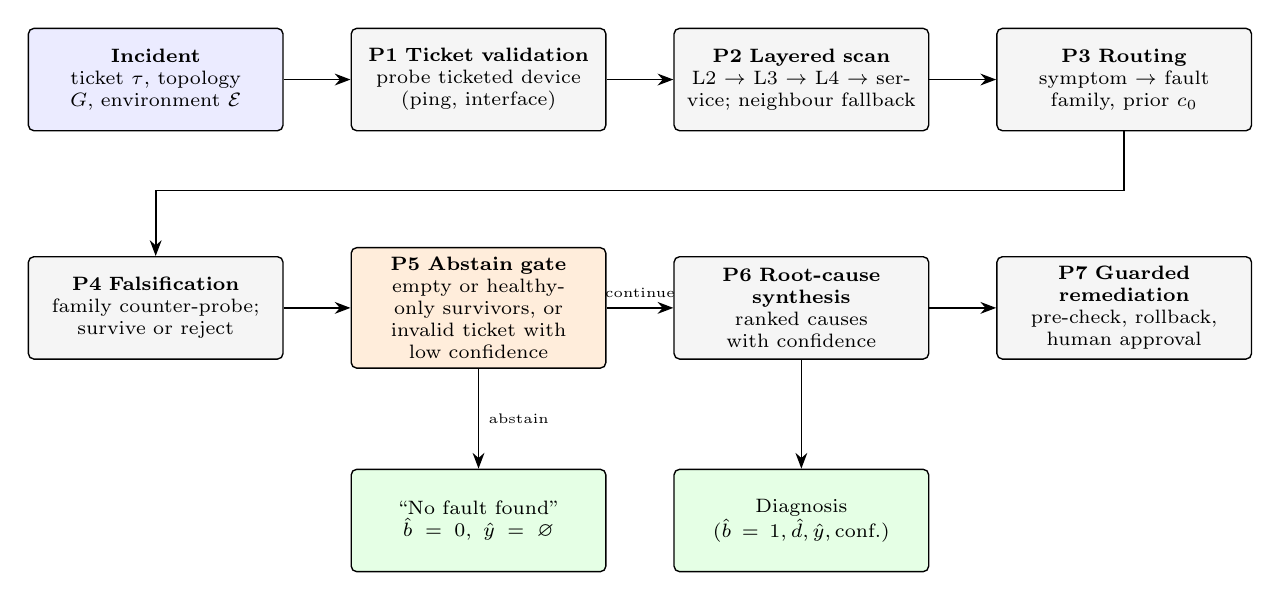
\begin{tikzpicture}[
  box/.style={draw, rounded corners=2pt, minimum height=1.3cm, text width=3.0cm, align=center, font=\scriptsize, fill=gray!8, line width=0.5pt},
  io/.style={box, fill=blue!8},
  gate/.style={box, fill=orange!14},
  outbox/.style={box, fill=green!10, text width=3.0cm},
  arr/.style={-{Stealth[length=2mm]}, line width=0.6pt}]
\node[io] (inc) at (0,0) {\textbf{Incident}\\ticket $\tau$, topology $G$, environment $\mathcal{E}$};
\node[box] (p1) at (4.1,0) {\textbf{P1 Ticket validation}\\probe ticketed device (ping, interface)};
\node[box] (p2) at (8.2,0) {\textbf{P2 Layered scan}\\L2 $\rightarrow$ L3 $\rightarrow$ L4 $\rightarrow$ service; neighbour fallback};
\node[box] (p3) at (12.3,0) {\textbf{P3 Routing}\\symptom $\rightarrow$ fault family, prior $c_0$};
\node[box] (p4) at (0,-2.9) {\textbf{P4 Falsification}\\family counter-probe; survive or reject};
\node[gate] (p5) at (4.1,-2.9) {\textbf{P5 Abstain gate}\\empty or healthy-only survivors, or invalid ticket with low confidence};
\node[box] (p6) at (8.2,-2.9) {\textbf{P6 Root-cause synthesis}\\ranked causes with confidence};
\node[box] (p7) at (12.3,-2.9) {\textbf{P7 Guarded remediation}\\pre-check, rollback, human approval};
\node[outbox] (no) at (4.1,-5.6) {``No fault found''\\$\hat b=0,\ \hat y=\varnothing$};
\node[outbox] (res) at (8.2,-5.6) {Diagnosis\\$(\hat b=1,\hat d,\hat y,\text{conf.})$};
\draw[arr] (inc) -- (p1); \draw[arr] (p1) -- (p2); \draw[arr] (p2) -- (p3);
\draw[arr] (p3.south) -- ++(0,-0.75) -| (p4.north);
\draw[arr] (p4) -- (p5); \draw[arr] (p5) -- node[above,font=\tiny]{continue} (p6); \draw[arr] (p6) -- (p7);
\draw[arr] (p5) -- node[right,font=\tiny]{abstain} (no);
\draw[arr] (p6) -- (res);
\end{tikzpicture}}\endgroup
\caption{Architecture of the seven-phase agent. Orange marks the abstain gate, which distinguishes the design from phase-gated agents that always return a fault. The agent never executes a remediation; phase 7 only produces a plan for human approval.}\label{fig:arch}
\end{figure*}

\paragraph{P1: ticket validation.} The ticketed device is the first device, in node order, whose lower-cased name is a substring of the lower-cased ticket (the first device $v_1$ if there is none),
\begin{equation}
d_\tau=\min\{v\in V:\ \mathrm{name}(v)\subseteq\mathrm{lower}(\tau)\}
\label{eq:ticketdev}
\end{equation}
Ping and interface probes are run on $d_\tau$. Let $\alpha(o)=1$ if the output shows packet loss, an unreachable or filtered destination, round-trip time above 100\,ms, or an interface down or in alarm. The ticket is \emph{valid} if $\alpha$ fires on either probe.

\paragraph{P2: layered scan.} For each layer in L2, L3, L4 and service, a fixed probe set is run on $d_\tau$, and rule extractors turn the trimmed output (500-token cap, repeated headers and whitespace removed) into evidence records $(\text{layer},\text{symptom},\text{severity},\text{snippet})$. If none is found and turns $<T-5$, the first neighbour of $d_\tau$ in $G$ is scanned and adopted if it yields evidence.

\paragraph{P3: routing.} Each record is matched against a fault-family index (the ``skill library''), producing hypotheses $h=(f,d,c_0)$ with prior
\begin{equation}
c_0=\begin{cases}0.70&\text{high severity}\\ 0.50&\text{otherwise}\\ 0.40&\text{generic fallback}\end{cases}
\label{eq:prior}
\end{equation}
and a family-specific counter-probe; the generic fallback is routing misconfiguration. With no evidence, the single hypothesis ``healthy'' with $c_0=0.95$ is produced.

\paragraph{P4: falsification.} For each non-healthy $h$ the counter-probe $\phi_f$ checks whether the output contradicts the claim (for example, a link-failure claim is contradicted by an interface whose line protocol is up). The survivors are $\mathcal{S}=\{h:\phi_f(h)=0\}$ and
\begin{equation}
c(h)=\begin{cases}0.05&\phi_f=1\ (\text{falsified})\\ \min(0.98,\ c_0+0.25)&\text{otherwise.}\end{cases}
\label{eq:conf}
\end{equation}

\paragraph{P5: abstain gate.} The agent reports $\hat b=0$ when
\begin{equation}
\begin{split}\text{abstain}=\mathbf{1}\Big[&\mathcal{S}=\varnothing\ \vee\ \mathcal{S}=\{\text{healthy}\}\\&\vee\ \big(\neg\,\text{valid}\ \wedge\ \max_{h\in\mathcal{S}}c(h)<0.50\big)\Big].\end{split}
\label{eq:abstain}
\end{equation}

\paragraph{P6 and P7: synthesis and remediation.} Survivors are ranked by $c(h)$; the top hypothesis $h^{*}$ gives $\hat y=f(h^{*})$ and $\hat d=d(h^{*})$, and the top three are returned with evidence. If $c(h^{*})\ge 0.80$, a family template with pre-check, post-check, rollback and risk level is attached and marked as requiring human approval. Remediation correctness is not evaluated in this study.

\begin{algorithm}[t]
\caption{Abstention-aware phase-gated troubleshooting}\label{alg:agent}
\raggedright\small
\begin{algorithmic}[1]
\Require ticket $\tau$, topology $G$, environment $\mathcal{E}$, budget $T$
\State $d\leftarrow d_\tau$ (Eq.~\ref{eq:ticketdev})
\State valid $\leftarrow\alpha(\text{ping}(d))\vee\alpha(\text{iface}(d))$
\State $\mathcal{R}\leftarrow\textsc{LayeredScan}(d)$
\If{$\mathcal{R}=\varnothing$ \textbf{and} turns $<T-5$}
  \State $u\leftarrow$ first neighbour of $d$
  \If{$\textsc{LayeredScan}(u)\neq\varnothing$}
    \State $d\leftarrow u$;\ $\mathcal{R}\leftarrow\textsc{LayeredScan}(u)$
  \EndIf
\EndIf
\State $H\leftarrow\textsc{Route}(\mathcal{R},d)$ \Comment{Eq.~\ref{eq:prior}}
\State $\mathcal{S}\leftarrow\{h\in H:\ \text{healthy}(h)\vee\phi_{f(h)}=0\}$, $c(h)$ by Eq.~\ref{eq:conf}
\If{abstain (Eq.~\ref{eq:abstain})}
  \State \Return $(0,\text{none},\varnothing)$
\EndIf
\State $h^{*}\leftarrow\arg\max_{h\in\mathcal{S}}c(h)$
\State \Return $(1,d(h^{*}),f(h^{*}))$, plus a guarded plan if $c(h^{*})\ge0.80$
\end{algorithmic}
\end{algorithm}

\subsection{Changes relative to the Phase 2 plan}\label{sec:changes}
The Phase 2 plan envisaged live emulation of NIKA and FaulT-Bench, several language-model backbones, repeated seeds and Wilcoxon tests. The study differs in five ways. (i) A deterministic Python simulator replaces the Kath\'ara emulator, trading realism for reproducibility. (ii) Only the rule-based path was run; the optional language-model client was disabled, so no backbone comparison exists. (iii) Repeated seeds give identical outputs, so variability is reported by bootstrap resampling of incidents, and exact McNemar tests replace the Wilcoxon test because outcomes are binary. (iv) The language-model judge score is excluded (Section~\ref{sec:threats}). (v) The ``large'' topologies have 17 to 77 nodes, not the planned 101.

\section{Experimental Setup}\label{sec:setup}

\paragraph{Simulator and corpus.} \texttt{MockNetworkEnv} returns deterministic command output per device; only the injected faulty device returns fault-specific telemetry, and every other device returns clean output. The 15 scenarios follow the NIKA families (data-centre CLOS, campus, ISP backbone, SDN cloud fabric, P4 testbed), eight FaulT-Bench-style topologies, an 11-node layout following the Internet2 Abilene backbone and a multi-tier enterprise topology labelled NetManAIOps. The last two reproduce only the topology shape with synthetic telemetry; no original dataset was used. Each scenario exists in three sizes (Table~\ref{tab:scen}, Appendix~\ref{secA1}).

The corpus holds 120 incidents. Ninety are faulty: scenario, size and fault family cycle deterministically, giving six faulty incidents per scenario, 12 or 13 per family and 30 per size. The ticket names the faulty device, except for every fifth incident (18 of 90), whose ticket names another device (a \emph{misdirected} ticket). Thirty are healthy controls with a false-premise ticket drawn from five reporter personas (panicked user, overconfident administrator, misdirected developer, monitoring-bot alarm, cautious operator); they exist in 10 of the 15 scenarios, three each, and their tickets name a device absent from the topology. A fault-injection audit confirmed that every injected fault produced the intended telemetry (120 of 120 passed).

\paragraph{Splits.} Scenarios are split as a whole. Ten scenarios (84 incidents: 60 faulty, 24 healthy) form the development partition and five (36 incidents: 30 faulty, 6 healthy) are held out: \texttt{p4\_testbed}, \texttt{sdn\_cloud\_fabric}, \texttt{bgp\_peering\_exchange}, \texttt{datacenter\_dci} and \texttt{abilene\_backbone}. No parameter is fitted to the data, since all thresholds are constants in the code (Table~\ref{tab:hyper}); the split therefore reveals behaviour on unseen scenarios rather than guarding model selection.

\paragraph{Baselines.} The five baselines are behavioural re-implementations, not the published systems, and none calls a language model here. \textbf{Zero-shot} maps ticket keywords to a family without probing. \textbf{ReAct-style} pings the ticketed device and takes the first keyword-matched symptom in a single reason-act loop~\cite{yao2023react}. \textbf{Coding-style} adds one scripted multi-command check. \textbf{SADE-style} follows the reachability scan, deep scan, family mapping and skill steps of SADE~\cite{tseng2026sade} without validation, falsification or abstention. \textbf{Scripted rules} run fixed checks with thresholds and can report ``no fault''. The first four always return a fault: with no anomaly they fall back to a default verdict. \emph{Their 100\% false-positive rate is therefore a property of their specification, not a measurement of the original systems.}

\paragraph{Metrics.} For incident $i$ let $\hat b_i,\hat d_i,\hat y_i$ be the output. \emph{Detection accuracy} is the share with $\hat b_i=b^{*}_i$; \emph{fault recall} is $\Pr(\hat b=1\mid b^{*}=1)$; the \emph{false-positive rate} (FPR) is $\Pr(\hat b=1\mid b^{*}=0)$; \emph{balanced accuracy} averages fault recall and $1-$FPR; \emph{localization accuracy} is $\Pr(\hat d=d^{*}\mid b^{*}=1)$. The \emph{RCA macro-F1} is
\begin{equation}
\mathrm{F1}_{\text{macro}}=\frac{1}{|\mathcal{L}|}\sum_{l\in\mathcal{L}}\frac{2\,\mathrm{TP}_l}{2\,\mathrm{TP}_l+\mathrm{FP}_l+\mathrm{FN}_l},
\label{eq:f1}
\end{equation}
with $\mathcal{L}$ the labels present in truth or predictions. Two variants are reported because the Phase 3 logs record the healthy truth as ``healthy'' while abstaining agents emit ``none''. \emph{As logged}, a correct abstention never matches; \emph{abstention credited} relabels ``healthy'' as ``none''. The second is the intended definition and is used in figures; the first is kept for continuity. A label-independent \emph{faulty-family F1} is macro-F1 over the seven families on the 90 faulty incidents, counting any ``none'' prediction as a miss. Efficiency is mean turns and modelled token counts (Section~\ref{sec:eff}).

\paragraph{Statistical protocol.} The pipeline is deterministic, so repeated runs are identical and no run-to-run standard deviation exists. Uncertainty is given by percentile bootstrap intervals over incidents (5,000 resamples, seed 20261117)~\cite{efron1993}. Paired differences use the same resamples and exact two-sided McNemar tests~\cite{mcnemar1947} on discordant incident pairs. No multiplicity correction is applied (a Bonferroni threshold for five baselines would be $0.01$). Incidents are generated cyclically and are not independent draws from a population, so intervals describe sampling variability within this corpus only.

\paragraph{Implementation.} The code is Python 3.12 with NetworkX~\cite{hagberg2008networkx}, SciPy~\cite{virtanen2020scipy} and scikit-learn~\cite{pedregosa2011sklearn}; figures use Matplotlib~\cite{hunter2007matplotlib}. The turn budget is 20, no language model is queried, and the full pipeline runs in about 5\,s on one CPU core. Table~\ref{tab:hyper} (Appendix~\ref{secA1}) lists all parameters and software versions.

\section{Results and Analysis}\label{sec:results}

\paragraph{Detection and false alarms.} Table~\ref{tab:detect} and Fig.~\ref{fig:main} report the 120-incident evaluation. The proposed agent raised no false alarm on the 30 healthy controls, whereas the four baselines without an abstention branch flagged all 30; the scripted rules also abstain correctly. The contrast is structural (Section~\ref{sec:setup}): it shows what an abstention branch changes in this simulator, not a measured weakness of the published systems. The price is recall. The agent detected 57 of 90 faults (63.3\%, 95\% CI [53.3, 73.2]), whereas the always-fault baselines detect all 90, so overall detection accuracy is indistinguishable (72.5\% against 75.0\% for SADE-style; exact McNemar $p=0.80$, 30 incidents won and 33 lost). Balanced accuracy is 81.7\%, against 50\% for any always-fault agent and 76.7\% for the scripted rules.

\begin{table*}[t]
\caption{Detection and false-alarm results on all 120 incidents (90 faulty, 30 healthy), in percent. Brackets are 95\% bootstrap intervals over incidents; intervals are degenerate for rates fixed at 0\% or 100\%.}\label{tab:detect}
\footnotesize
\begin{tabular}{@{}lcccc@{}}
\toprule
Agent & Detection acc. & Fault recall & FPR & Balanced acc. \\
\midrule
Zero-shot & 75.0 [66.7, 82.5] & 100.0 & 100.0 & 50.0 [50.0, 50.0] \\
ReAct-style & 75.0 [66.7, 82.5] & 100.0 & 100.0 & 50.0 [50.0, 50.0] \\
Coding-style & 75.0 [66.7, 82.5] & 100.0 & 100.0 & 50.0 [50.0, 50.0] \\
SADE-style & 75.0 [66.7, 82.5] & 100.0 & 100.0 & 50.0 [50.0, 50.0] \\
Scripted rules & 65.0 [56.7, 73.3] & 53.3 & 0.0 & 76.7 [71.4, 81.7] \\
\textbf{Proposed} & 72.5 [64.2, 80.0] & 63.3 & 0.0 & 81.7 [76.6, 86.6] \\
\botrule
\end{tabular}
\end{table*}

\begin{figure*}[t]
\centering
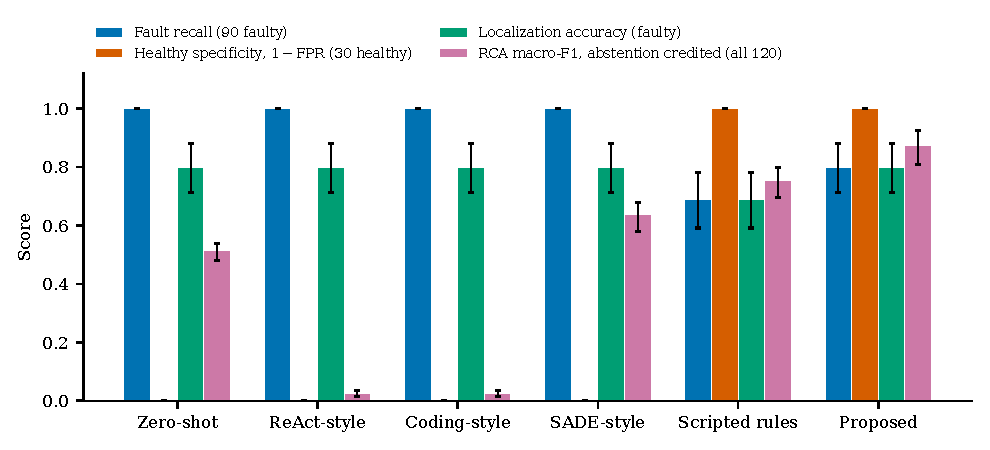
\includegraphics[width=\linewidth]{figures/fig_main_results.pdf}
\caption{Diagnostic results per agent on 120 incidents: fault recall, healthy specificity ($1-$FPR), localization accuracy and root-cause macro-F1 with abstentions credited. Error bars are 95\% bootstrap intervals over incidents. The four baselines without an abstention branch have zero specificity by construction.}\label{fig:main}
\end{figure*}

\paragraph{Localization and root cause.} Localization accuracy is 63.3\% for the proposed agent and for every baseline that parses the ticket (Table~\ref{tab:rca}), because all take the device from the same ticket-parsing step: in 57 of 90 faulty incidents the ticket points to the true device, and no agent recovers from a wrong ticket. Localization is thus dominated by ticket handling, not diagnostic reasoning (Section~\ref{sec:failure}).

\begin{table*}[t]
\caption{Localization and root-cause results. Accuracy on faulty incidents is exact family match. Macro-F1 is given as logged and with abstention credited; faulty-family F1 is label-independent. Brackets are 95\% bootstrap intervals.}\label{tab:rca}
\scriptsize
\begin{tabular}{@{}lccccc@{}}
\toprule
Agent & Loc. (\%) & RCA acc. faulty (\%) & Faulty-family F1 & F1 as logged & F1 credited \\
\midrule
Zero-shot & 63.3 & 72.2 & 0.644 [0.619, 0.667] & 0.513 & 0.513 [0.479, 0.539] \\
ReAct-style & 63.3 & 14.4 & 0.036 [0.021, 0.052] & 0.024 & 0.024 [0.014, 0.036] \\
Coding-style & 63.3 & 14.4 & 0.036 [0.021, 0.052] & 0.024 & 0.024 [0.014, 0.036] \\
SADE-style & 63.3 & 57.8 & 0.650 [0.556, 0.722] & 0.560 & 0.560 [0.481, 0.618] \\
Scripted rules & 53.3 & 53.3 & 0.658 [0.567, 0.721] & 0.512 & 0.649 [0.565, 0.712] \\
\textbf{Proposed} & 63.3 & 63.3 & 0.775 [0.678, 0.842] & 0.602 & 0.758 [0.668, 0.827] \\
\botrule
\end{tabular}
\end{table*}

With abstention credited, the proposed agent's macro-F1 is 0.758 (95\% CI 0.668--0.827), against 0.560 for SADE-style, 0.649 for the scripted rules and 0.513 for zero-shot. As logged it is only 0.602, because correct abstentions are not matched to the healthy label; crediting them adds about 0.16. On genuine faults alone, the label-independent faulty-family F1 is 0.775 (CI [0.678, 0.842]) against 0.650 (CI [0.556, 0.722]) for SADE-style; the intervals overlap, and the paired test on faulty-incident family accuracy is not significant against SADE-style (9/4 incidents won/lost, $p=0.27$) or zero-shot ($p=0.26$). Zero-shot even has higher raw faulty accuracy (72.2\% against 63.3\%): keyword matching works when the ticket wording is distinctive, whereas the proposed agent abstains on 33 faulty incidents. The ReAct-style and Coding-style agents reach only 14.4\% because they output ``congestion'' for every incident (13 of 90 faulty incidents are congestion); they are degenerate constant predictors of the re-implementation, not representative ReAct agents. Recall of the proposed agent is uniform across families (53.8\% to 69.2\%).

\paragraph{Statistical evidence.} Table~\ref{tab:paired} gives paired comparisons. The abstention gain is highly significant: the proposed agent is right on all 30 healthy controls where the four always-fault baselines are wrong. On faulty incidents it beats the scripted rules (9 won, 0 lost, $p=0.004$) and the ReAct-style and Coding-style agents (49 against 5), but not SADE-style or zero-shot. The bootstrap interval for the macro-F1 gain over SADE-style excludes zero only with abstention credited (+0.198, CI [+0.143, +0.242]); as logged it is +0.042 (CI [-0.004, +0.080]).

\begin{table*}[t]
\caption{Paired comparison of the proposed agent with each baseline. $\Delta$F1 is proposed minus baseline macro-F1 with a 95\% bootstrap interval. The last three columns give won/lost incident counts (exact McNemar $p$) on the 30 healthy controls, on detection correctness for all 120 incidents, and on family correctness for the 90 faulty incidents.}\label{tab:paired}
\scriptsize
\begin{tabular}{@{}L{1.5cm}L{3.4cm}L{3.4cm}L{2.0cm}L{2.0cm}L{1.9cm}@{}}
\toprule
Baseline & $\Delta$F1 credited & $\Delta$F1 as logged & Healthy controls & Detection & RCA, faulty \\
\midrule
Zero-shot & +0.245 [+0.148, +0.322] & +0.089 [+0.013, +0.151] & 30/0 ($<0.001$) & 30/33 (0.801) & 15/23 (0.256) \\
ReAct-style & +0.734 [+0.644, +0.801] & +0.578 [+0.507, +0.631] & 30/0 ($<0.001$) & 30/33 (0.801) & 49/5 ($<10^{-9}$) \\
Coding-style & +0.734 [+0.644, +0.801] & +0.578 [+0.507, +0.631] & 30/0 ($<0.001$) & 30/33 (0.801) & 49/5 ($<10^{-9}$) \\
SADE-style & +0.198 [+0.143, +0.242] & +0.042 [-0.004, +0.080] & 30/0 ($<0.001$) & 30/33 (0.801) & 9/4 (0.267) \\
Scripted rules & +0.109 [+0.079, +0.130] & +0.091 [+0.067, +0.107] & 0/0 (1.000) & 9/0 (0.004) & 9/0 (0.004) \\
\botrule
\end{tabular}
\end{table*}

\paragraph{Held-out scenarios and topology size.} On the five held-out scenarios the proposed agent's recall falls from 70.0\% (development) to 50.0\%, detection accuracy from 78.6\% to 58.3\%, and credited macro-F1 from 0.813 to 0.633 (Fig.~\ref{fig:split}); SADE-style falls from 0.598 to 0.472. With only 30 faulty and 6 healthy held-out incidents, these differences are uncertain, and every fault family appears in both partitions. Per-scenario detection accuracy has mean $\pm$ standard deviation 71.1 $\pm$ 37.5\% for the proposed agent, 77.8 $\pm$ 16.3\% for SADE-style and 63.3 $\pm$ 32.9\% for the scripted rules; the larger spread reflects four scenarios in which the agent detects none of six faults, where misdirected tickets and name collisions coincide. Recall is 80.0\%, 80.0\% and 30.0\% on small, medium and large topologies; the collapse at large size comes from name collisions in the ticket parser, not from scale in the diagnostic logic (Section~\ref{sec:failure}).

\begin{figure*}[t]
\centering
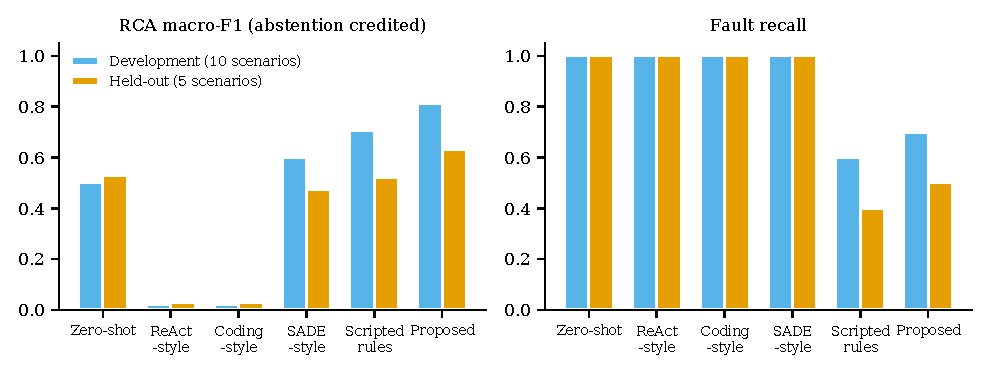
\includegraphics[width=\linewidth]{figures/fig_split_transfer.pdf}
\caption{Development versus held-out scenarios: root-cause macro-F1 with abstention credited (left) and fault recall (right). Held-out scenarios contain 30 faulty and 6 healthy incidents.}\label{fig:split}
\end{figure*}

\paragraph{Efficiency.}\label{sec:eff} Token counts are accounting constants of the simulator (fixed increments per phase), not API measurements, and the Phase 3 logs priced agents on different schedules. Table~\ref{tab:eff} therefore re-prices all agents at one schedule (USD 0.003 per 1k input, 0.015 per 1k output tokens). The proposed agent needs 8.69 turns on average against 6.00 for SADE-style and costs 1.13 times as much as SADE-style (USD 0.0124 against 0.0110 per incident) and 3.2 times as much as ReAct-style, the price of its validation and falsification probes. These figures say nothing about the cost of published language-model agents.

\begin{table}[t]
\caption{Mean turns, modelled tokens per incident (input / output) and modelled cost in USD per 1,000 incidents at a common price schedule.}\label{tab:eff}
\footnotesize
\begin{tabular}{@{}lccc@{}}
\toprule
Agent & Turns & Tokens in/out & Cost \\
\midrule
Zero-shot & 1.00 & 143 / 60 & 1.33 \\
ReAct-style & 1.00 & 670 / 120 & 3.81 \\
Coding-style & 2.00 & 950 / 400 & 8.85 \\
SADE-style & 6.00 & 1550 / 420 & 10.95 \\
Scripted rules & 4.00 & 0 / 0 & 0.00 \\
\textbf{Proposed} & 8.69 & 1760 / 471 & 12.35 \\
\botrule
\end{tabular}
\end{table}

\section{Comparison with Base Papers and State of the Art}\label{sec:base}

The work builds on three base papers: NIKA for scenario families and tool vocabulary, SADE for the phase-gated policy and the strongest baseline, and FaulT-Bench for healthy controls and false-premise tickets. BiAn and Confucius contribute SOP-style heuristics and the validation gate. Table~\ref{tab:basesum} summarises them.

\begin{table*}[t]
\caption{Summary of the base papers and the strongest supporting study.}\label{tab:basesum}
\scriptsize
\begin{tabular}{@{}L{1.7cm}L{2.0cm}L{2.2cm}L{2.1cm}L{1.7cm}L{2.3cm}L{1.9cm}@{}}
\toprule
Paper & Problem & Method & Data & Metrics & Reported results & Limitations \\
\midrule
NIKA, Wang et al. 2025~\cite{wang2025nika} & Reproducible comparison of troubleshooting agents & Emulated incidents; MCP tools; ReAct reference agents & 640 incidents, 54 issues, 5 scenarios (150 evaluated) & Detection, localization, RCA accuracy; steps; tokens & GPT-5: 89.0 / 68.7 / 55.3\% & Emulation only; no healthy cases; no mitigation \\
SADE, Tseng et al. 2026~\cite{tseng2026sade} & Early hypothesis commitment of free-form agents & Phase-gated escalation, 15 skills, Claude Sonnet 4.6 & 523 held-out NIKA incidents & RCA F1; detection; judge; tokens & F1 0.77 vs 0.55 (same-model coding agent); detection 0.85 & Hand-written skills; injector defects; cost \\
FaulT-Bench, Tseng et al. 2026~\cite{tseng2026faultbench} & Agents under unreliable tickets & 200 scenarios, 8 topologies, personas; LLM judge & Emulated, with false reports and healthy networks & Outcome, fix, reasoning (judge) & Near saturation on accurate tickets; sharp drop on healthy network with wrong ticket & Modest scale; LLM judge; no remedy \\
BiAn, Wang et al. 2025~\cite{wang2025bian} & Device localization in production cloud & SOP-guided agents, topology and event pipelines & Proprietary, 357 incidents & Accuracy; time to root cause & 95.5\% vs 86.3\% baseline & Closed data; device level \\
\botrule
\end{tabular}
\end{table*}

\paragraph{Quantitative comparison.} Table~\ref{tab:quant} places the simulated results beside the published numbers, but \emph{the two groups of rows are not comparable}: published values (asterisk) come from language-model backends on emulated incidents with other incident sets and metric definitions, whereas our rows come from this study's simulator and all our baselines are re-implementations. No original code or number of the base papers was reproduced.

\begin{table*}[t]
\caption{Quantitative comparison. Rows marked $^{*}$ are numbers from the original papers (different environment and metrics; not comparable). Rows marked $^{\dagger}$ are re-implementations in this study's simulator ($n=120$). Detection and localization in percent; n/r = not reported in the material reviewed. Where two F1 values are given, they are as logged / abstention credited.}\label{tab:quant}
\scriptsize
\begin{tabular}{@{}L{4.2cm}L{1.4cm}L{1.8cm}L{1.5cm}L{2.3cm}L{2.2cm}@{}}
\toprule
Agent (environment) & Detection & Localization & FPR healthy & Root-cause score & Cost \\
\midrule
ReAct, GPT-5$^{*}$ (NIKA emulator) \cite{wang2025nika} & 89.0 & 68.7 & n/r & 55.3\% accuracy & n/r \\
SADE, Claude Sonnet 4.6$^{*}$ (NIKA) \cite{tseng2026sade} & 85 & n/r & n/r & F1 0.77 & about USD 1.44 per session \\
Coding agent, same model$^{*}$ \cite{tseng2026sade} & about 67 & n/r & n/r & F1 0.55 & n/r \\
ReAct, GPT-5$^{*}$ \cite{tseng2026sade} & n/r & n/r & n/r & F1 0.40--0.44 & about USD 0.20 per session \\
\midrule
ReAct-style$^{\dagger}$ (simulator) & 75.0 & 63.3 & 100.0 & F1 0.024 & modelled \\
SADE-style$^{\dagger}$ (simulator) & 75.0 & 63.3 & 100.0 & F1 0.560 & modelled \\
Scripted rules$^{\dagger}$ (simulator) & 65.0 & 53.3 & 0.0 & F1 0.512 / 0.649 & none \\
\textbf{Proposed}$^{\dagger}$ (simulator) & 72.5 & 63.3 & 0.0 & F1 0.602 / 0.758 & modelled \\
\botrule
\end{tabular}
\end{table*}

The proposed agent's detection, localization and F1 are numerically lower than the published SADE and NIKA figures, which is expected and uninformative: the simulator misdirects 20\% of tickets, the agent cannot recover from them, and the metric definitions differ. The only conclusion drawn is qualitative: abstention removes false alarms on healthy controls and costs recall when the ticket cannot be trusted. The agent does not outperform the base papers on any comparable metric.

\paragraph{Methodological comparison.} Relative to SADE, the agent adds ticket validation, active falsification and an abstain gate, and replaces the language-model skill library by an explicit rule index. Relative to NIKA it adds healthy controls and a false-positive metric. Relative to FaulT-Bench it proposes an agent aimed at the identified over-diagnosis, though it is tested only on perfectly clean healthy networks. Relative to Confucius it adopts gated, human-approved actions but implements only a plan. Relative to RCLAgent it uses bounded evidence, but the simulator's short outputs make trimming immaterial (Section~\ref{sec:ablation}).

\paragraph{Improvement analysis.} Table~\ref{tab:improve} gives absolute and relative changes against three re-implemented baselines. The gain in credited macro-F1 over SADE-style (0.198, 35.4\% relative) arises almost entirely from the healthy class: the 30 healthy incidents move from wrong to right. On genuine faults the gain is the smaller faulty-family F1 difference (+0.125), and the paired accuracy test is not significant ($p=0.27$). The gain over the scripted rules (+0.109, 16.9\%) is the most robust: the agent detects 10 points more faults while abstaining equally well ($p=0.004$). All gains are paid for in fault recall relative to the always-fault baselines ($-36.7$ points).

\begin{table*}[t]
\caption{Change of the proposed agent relative to three re-implemented baselines: absolute change, with relative change in parentheses (pp = percentage points). A negative false-positive change is an improvement.}\label{tab:improve}
\scriptsize
\begin{tabular}{@{}lccc@{}}
\toprule
Metric & vs.\ SADE-style & vs.\ Scripted rules & vs.\ Zero-shot \\
\midrule
Detection accuracy (pp) & -2.5 (-3.3\%) & +7.5 (+11.5\%) & -2.5 (-3.3\%) \\
Fault recall (pp) & -36.7 (-36.7\%) & +10.0 (+18.7\%) & -36.7 (-36.7\%) \\
False-positive rate (pp) & -100.0 (-100.0\%) & +0.0 (n/a) & -100.0 (-100.0\%) \\
Localization accuracy (pp) & +0.0 (+0.0\%) & +10.0 (+18.7\%) & +0.0 (+0.0\%) \\
RCA macro-F1, as logged & +0.042 (+7.6\%) & +0.091 (+17.8\%) & +0.089 (+17.4\%) \\
RCA macro-F1, abstention credited & +0.198 (+35.4\%) & +0.109 (+16.9\%) & +0.245 (+47.8\%) \\
Faulty-family F1 (7 families) & +0.125 (+19.2\%) & +0.117 (+17.8\%) & +0.130 (+20.2\%) \\
\botrule
\end{tabular}
\end{table*}

\paragraph{Fairness.} Four factors limit the comparison. (i) The baselines are specified by this study's authors and can be made weaker or stronger by design; the 100\% FPR is an instance. (ii) All agents share one simulator, ticket parser and metric definition, which is fair among them but unlike the base papers' settings. (iii) The agent's rules and the simulator's telemetry strings were written by the same team and share vocabulary (for example ``NO-CARRIER'' and ``Null0''), so accuracy on correctly parsed incidents is 100\% by construction. (iv) Token and cost figures are modelled.

\section{Ablation Study}\label{sec:ablation}
Six variants were re-executed on a separate 60-incident corpus (42 faulty, 18 healthy) with the same code and per-incident logs; their summary metrics reproduce the Phase 3 ablation file. Table~\ref{tab:abl} and Fig.~\ref{fig:abl} report them.

\begin{table*}[t]
\caption{Ablation on 60 incidents (42 faulty, 18 healthy); rates in percent. F1 columns follow Section~\ref{sec:setup}.}\label{tab:abl}
\scriptsize
\begin{tabular}{@{}L{3.0cm}L{5.2cm}cccc c@{}}
\toprule
Variant & Change & Recall & FPR & Loc. & F1 logged & F1 credited \\
\midrule
Full agent & -- & 66.7 & 0.0 & 66.7 & 0.617 & 0.784 \\
$-$ Evidence filtering & trimming to 500 tokens off & 66.7 & 0.0 & 66.7 & 0.617 & 0.784 \\
$-$ Abstain gate & abstention (and fast path) off & 100.0 & 100.0 & 66.7 & 0.784 & 0.617 \\
$-$ Falsification & all hypotheses survive unchallenged & 45.2 & 0.0 & 45.2 & 0.311 & 0.426 \\
$-$ Skill library & single generic hypothesis & 100.0 & 0.0 & 66.7 & 0.028 & 0.156 \\
$-$ Phase gating & validation, falsification, abstain, filtering, skills all off & 100.0 & 100.0 & 21.4 & 0.023 & 0.023 \\
\botrule
\end{tabular}
\end{table*}

\begin{figure*}[t]
\centering
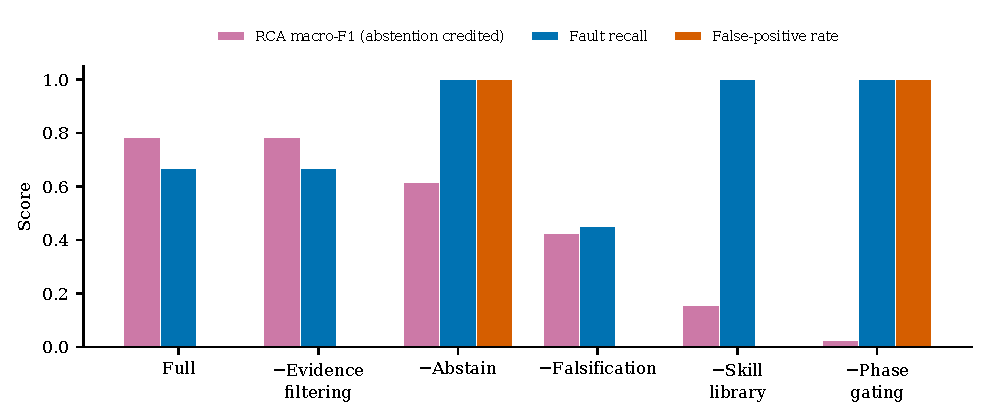
\includegraphics[width=\linewidth]{figures/fig_ablation.pdf}
\caption{Ablation of the proposed agent on 60 incidents: root-cause macro-F1 with abstention credited, fault recall and false-positive rate per variant.}\label{fig:abl}
\end{figure*}

\textbf{Abstain gate.} Removing it raises recall and FPR to 100\%. As logged, macro-F1 appears to \emph{improve} (0.784 against 0.617); with abstentions credited the order reverses (0.617 against 0.784), so the logged comparison is an artefact of the label mismatch. \textbf{Falsification.} Disabling the counter-probes lowers recall from 66.7\% to 45.2\% and credited F1 from 0.784 to 0.426. All nine lost detections are service or DNS failures: ping and interface probes cannot see them, so their tickets fail validation, and they pass the abstain gate only because surviving a counter-probe raises their confidence. \textbf{Skill library.} A single generic hypothesis gives credited F1 0.156: detection is perfect because everything is reported as a fault, but the root cause is almost always wrong. \textbf{Phase gating.} Removing all structure yields credited F1 0.023; this is a floor rather than a single-component effect, since with validation off the agent also probes the first topology device instead of the ticketed one. \textbf{Evidence filtering.} Disabling trimming changes nothing: simulator outputs are shorter than the 500-token cap, so the evidence-dilution effect reported for real agents~\cite{zhang2026rclagent} cannot be tested here.

\section{Discussion}\label{sec:discussion}

\paragraph{Why it works, and what it implies.} In the simulator, healthy devices return clean telemetry and each family has a distinctive signature, so an agent that checks the ticketed device, probes upward and then tries to refute its finding can recognise a healthy network and reject spurious families. The ablations agree: the skill library and falsification carry the diagnostic load and the abstain gate accounts for the whole change in false alarms. For operators the results expose a usually hidden trade-off: an agent that always answers wastes effort on healthy networks, whereas one that abstains risks missing real faults when the ticket misleads. A deployment must decide how to treat an \emph{invalid} ticket, for example by escalating to a wider scan instead of abstaining. Strengths of the study are auditable rules, regeneration in seconds on one core, healthy controls with a whole-scenario holdout, paired tests, a leakage audit and a complete attribution of the agent's misses.

\subsection{Failure analysis}\label{sec:failure}
Of 90 faulty incidents the agent misses 33, each with a single identified cause (Fig.~\ref{fig:fail}). Eighteen carry a \emph{misdirected ticket}: the ticketed device is healthy, validation finds no anomaly, the ticket is judged invalid and the agent abstains, so recall on misdirected tickets is 0 of 18. Fifteen are \emph{device-name collisions} in the large topologies: Eq.~(\ref{eq:ticketdev}) takes the first device whose name is a substring of the ticket, so a ticket naming \texttt{access\_sw10} resolves to \texttt{access\_sw1}. When the ticketed device is parsed correctly and correct, the agent detects 57 of 57 faults and names the right family every time. The 63.3\% recall and the apparent scale effect are therefore properties of ticket handling. Misdirection is the harder issue: FaulT-Bench found real agents largely robust to wrong device attribution, so the zero recall here is a design weakness. The collision is an implementation defect; whole-token matching would remove it, and if the 15 affected faults were then detected as the 57 correctly parsed ones were, recall would reach 80\%. This is a projection from the logs, not a measured result.

\begin{figure*}[t]
\centering
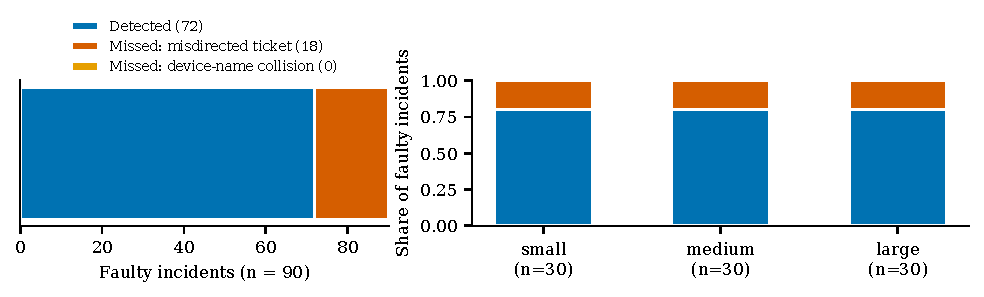
\includegraphics[width=\linewidth]{figures/fig_failure_attribution.pdf}
\caption{Outcomes of the 90 faulty incidents for the proposed agent. Left: detected incidents and the two causes of misses. Right: the same breakdown by topology size; collisions occur only in the large topologies.}\label{fig:fail}
\end{figure*}

\subsection{Limitations and threats to validity}\label{sec:threats}
\textbf{Simulation and circularity.} The environment, ticket generator and agent rules were written by one team around one vocabulary, so results describe behaviour on this simulator and cannot be extrapolated to emulators or production. Healthy controls are perfectly clean; real healthy networks show noise and partial degradation, so a zero false-positive rate is optimistic. \textbf{No language model.} The evaluated agent is rule-based; backbone effects, prompt variation and hallucination~\cite{kim2026agents} were not measured. \textbf{Baselines by construction.} Four baselines return a fault by specification, so their FPR and the corresponding F1 gains are structural; only the scripted rules give a non-trivial abstaining comparison. \textbf{Labels and metrics.} The healthy-label mismatch changes the logged F1 of abstaining agents. The Phase 3 judge score was excluded: its rubric is hand-coded and its values differ between the committed run and a re-execution of the same code, while all diagnostic metrics reproduce exactly. Token counts are fixed constants. \textbf{Ground-truth leakage.} The orchestrator has a fast path that reads the simulator's healthy-control flag; hiding the flag changes none of the 120 outputs, so results are unaffected, but the path should be removed. \textbf{Statistical dependence.} Incidents are generated cyclically and are not independent samples, and the held-out partition has only six healthy incidents. The Phase 3 persona stress test did not vary agent behaviour (no agent reads the persona beyond device names), so no robustness to ticket style is claimed.

\subsection{Were the research gap and objectives met?}
\textbf{Sub-gap A (healthy controls):} partly. Controls and an abstention mechanism were implemented and removed all false alarms, but only in a clean simulator against baselines that cannot abstain. \textbf{Sub-gap B (complete metrics):} largely. Detection, localization, family accuracy, F1, FPR, steps and modelled tokens are reported with intervals; real token cost and time to diagnosis were not obtained. \textbf{Sub-gap C (transfer):} partly. A whole-scenario holdout was evaluated and performance dropped; cross-domain transfer was not tested. The objective of a reproducible agent and protocol is met; demonstrating improvement on realistic benchmarks is not.

\section{Conclusion and Future Work}\label{sec:conclusion}
This paper presented an abstention-aware, phase-gated troubleshooting agent and a reproducible simulated protocol with healthy controls, whole-scenario holdout and paired statistics. In the simulator the agent raised no false alarm on 30 healthy controls and reached a credited root-cause macro-F1 of 0.758 at a fault recall of 63.3\%; ablations identify falsification and the fault-family index as the key components. Against the strongest re-implemented baseline the gain on genuine faults is not significant, and every missed fault stems from a misdirected ticket or a name-matching defect. Future work should (i) fix the ticket parser and add recovery for misdirected tickets, such as a wider scan on invalid tickets; (ii) move to the Kath\'ara-based NIKA and FaulT-Bench environments with noisy healthy networks; (iii) evaluate language-model backbones and measure real token cost; (iv) correct the label mismatch and report both F1 variants in all runs; and (v) evaluate remediation plans against the gates they promise.

\backmatter

\bmhead{Supplementary information}
Per-incident run logs, ablation logs, analysis scripts and figure sources accompany the paper (Appendix~\ref{secA1}).

\section*{Declarations}
\begin{itemize}
\item \textbf{Funding.} No external funding was received.
\item \textbf{Conflict of interest.} The authors declare no competing interests.
\item \textbf{Ethics approval and consent to participate; consent for publication.} Not applicable.
\item \textbf{Data availability.} All data are synthetic and generated by the released code; per-incident logs are in the repository (\texttt{results/raw\_runs.csv}).
\item \textbf{Code availability.} Code, configuration, logs and analysis scripts are in the project repository [repository URL to be inserted by the authors before submission]. The credential of the optional language-model client must be supplied through an environment variable and is not part of the release.
\item \textbf{Author contribution.} A.A. and T.A. designed the study, implemented the agent and baselines and ran the experiments.
\item \textbf{AI-tool usage declaration.} An AI assistant (Claude, Anthropic) helped draft the text and LaTeX source of this manuscript, re-analysed the logged results (bootstrap intervals, paired tests, failure attribution, leakage audit) and generated the figures from those logs. Every reported number was checked against the logged outputs, and the authors take full responsibility for the content. This statement should be extended if AI tools were also used to write the code.
\end{itemize}

\begin{appendices}

\section{Reproducibility details}\label{secA1}
\textbf{Code and data.} The simulator, agent, baselines and runner are in \texttt{code/}; configuration is in \texttt{configs/experiment\_config.yaml} and \texttt{configs/splits.json}. \texttt{python run\_all.py --skip\_pdf} rebuilds \texttt{results/raw\_runs.csv}, the metric summary and the ablation file in about 5\,s on one CPU core without network access. The scripts \texttt{analysis/phase4\_analysis.py}, \texttt{ablation\_rerun.py}, \texttt{leakage\_audit.py} and \texttt{build\_tables.py} derive every number, figure and table of this paper from the logs. \textbf{Verification.} Detection accuracy, recall, localization, FPR and both F1 variants were identical between the committed Phase 3 result files and a fresh re-execution; columns that depend on the optional language-model client (token counts of some baselines, wall-clock time, judge score) differed and support no claim. The 32 unit tests of the repository pass. \textbf{Seeds.} No agent uses randomness; the healthy-control generator uses seed 42 and the bootstrap seed 20261117.

\begin{table*}[h]
\caption{Scenario composition. Node counts are given for the small/medium/large topology variants.}\label{tab:scen}
\footnotesize
\begin{tabular}{@{}llcccc@{}}
\toprule
Scenario & Family & Split & Faulty & Healthy & Nodes \\
\midrule
\texttt{abilene\_backbone} & Course: Abilene & Held-out & 6 & 0 & 11/33/77 \\
\texttt{bgp\_peering\_exchange} & FaulT-Bench & Held-out & 6 & 0 & 6/8/18 \\
\texttt{campus\_core\_access} & FaulT-Bench & Dev. & 6 & 0 & 6/8/18 \\
\texttt{campus\_network} & NIKA & Dev. & 6 & 3 & 6/8/18 \\
\texttt{datacenter\_clos} & NIKA & Dev. & 6 & 3 & 10/15/40 \\
\texttt{datacenter\_dci} & FaulT-Bench & Held-out & 6 & 0 & 10/15/40 \\
\texttt{enterprise\_branch} & FaulT-Bench & Dev. & 6 & 3 & 6/8/18 \\
\texttt{isp\_backbone} & NIKA & Dev. & 6 & 3 & 6/9/24 \\
\texttt{leaf\_spine\_clos} & FaulT-Bench & Dev. & 6 & 3 & 10/15/40 \\
\texttt{multihomed\_edge} & FaulT-Bench & Dev. & 6 & 3 & 6/8/18 \\
\texttt{netman\_aiops} & Course: NetManAIOps & Dev. & 6 & 0 & 13/15/25 \\
\texttt{p4\_testbed} & NIKA & Held-out & 6 & 3 & 6/8/18 \\
\texttt{sdn\_cloud\_fabric} & NIKA & Held-out & 6 & 3 & 5/7/17 \\
\texttt{sdn\_hybrid} & FaulT-Bench & Dev. & 6 & 3 & 5/7/17 \\
\texttt{transit\_wan} & FaulT-Bench & Dev. & 6 & 3 & 6/9/24 \\
\midrule
Total & & & 90 & 30 & \\
\botrule
\end{tabular}
\end{table*}

\begin{table*}[h]
\caption{Fixed parameters and environment of the reported runs.}\label{tab:hyper}
\footnotesize
\begin{tabular}{@{}L{5.0cm}L{10.5cm}@{}}
\toprule
Item & Value \\
\midrule
Turn budget $T$ & 20 (neighbour fallback only if turns $<T-5$) \\
Hypothesis priors $c_0$ & 0.70 (high severity), 0.50, 0.40 (fallback), 0.95 (healthy) \\
Survival boost / cap / falsified & $+0.25$ / 0.98 / 0.05 \\
Abstain threshold (invalid ticket) & 0.50 \\
Remediation confidence gate & 0.80, human approval always required \\
Latency threshold in $\alpha(\cdot)$ & 100\,ms \\
Tool-output trimming & 500 tokens, headers and whitespace normalised \\
Language model & none queried (client for \texttt{gemini-1.5-flash}, temperature 0.1, disabled) \\
Random seeds & none needed for agents; healthy-control generator seed 42; bootstrap seed 20261117 \\
Hardware, runtime & single CPU core, Linux x86-64 container; full pipeline about 5\,s \\
Software & Python 3.12.3, NetworkX 3.7, NumPy 2.5.4, pandas 3.0.6, SciPy 1.18.1, scikit-learn 1.9.1, Matplotlib 3.11.2 \\
\botrule
\end{tabular}
\end{table*}

\end{appendices}

\bibliography{references}

\end{document}
